
With the goal of topographical mapping in mind, refinement of scope and the establishment of a plan was required. 

\subsection{Scope}
In the real world, topographical drone applications would require the ability to traverse large areas across many environments while encountering obstacles of unknown and drastically varying size. The team recognized immediately that the scope of the project needed to be refined first to ensure that a feasible goal was established. 

\subsubsection{Grid and Flight Pattern}
First, it was decided that a fixed test space was needed such that it balanced room for adequate data collection and the ability to rapidly iterate. Too large of an area would take too long to fly over and would require more free space, while too small of an area wouldn't provide enough flight time and could potentially lead to minimal space to perform maneuvers. A 1.5 meter square grid was selected as the test space.

A space-driven flight pattern was then created and standardized to be used across all tests performed. This was another instance of refining scope - though in the real world drones may fly in unique patterns with complex maneuvers, this predetermined flight path allows for simplicity and repeat-ability. The drone was flown at a constant height of 0.45 meters, taking off from the origin and completing a forward lawnmower pattern of fixed width across the grid. Once complete, the drone would engage in a reverse lawnmower pattern, flying again in fixed-width sweeps back to the origin where it would land. The grid and flight path are shown below in Figure \ref{fig:lawnmower}. The
drone begins at the bottom left corner which was be defined as the origin (0,0). The end of the grid in coordinate system
is (1.5,1.5). The dark blue lines depict the path of the drone moving forward to the end of the grid. The red dashed line depicts the drone returning back to origin from the end.

\begin{figure}[H]
  \centering
  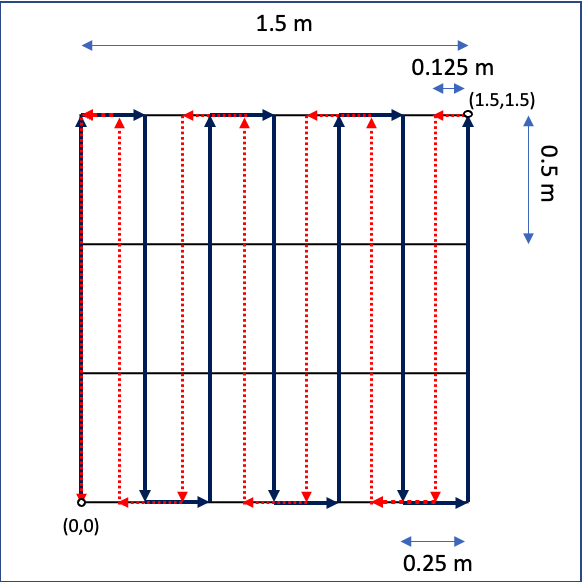
\includegraphics[width=0.6\linewidth, height=0.6\linewidth]{Technical/FP.png}  
  \caption{Drone forward (navy) and backward (red) lawnmower flight pattern on square grid}
  \label{fig:lawnmower}
\end{figure}

\subsubsection{Obstacles and Object Detection}
By the nature of their application, drones used for topographical mapping are collecting data on objects of unknown dimensions. Inherently, drones that are flying close to the objects of interest must be equipped with obstacle avoidance capabilities such that they do not collide with the things they are studying. To minimize this added level of complexity, the project scope was refined to only detect objects' dimensions, rather than also actively try to avoid them. To do this, objects of known dimensions were used in this study which allowed the aforementioned constant flight height to be set at a value higher than the tallest obstacle. This ensured that the drone was always flying high enough to never crash into an object. In addition to simplifying obstacle avoidance, having objects of known dimensions gave a baseline to compare drone mapping results against to gauge topographical measurement accuracy.

The number of objects on the grid was set to two, each being detected twice in one flight loop - once during the forward lawnmower sweep and again in the backward sweep. This was done to ensure that the test space wasn't over crowded, and that adequate spacing would allow for clear contrast of measured object heights relative to what was being detected as the floor. It would have been undesirable to produce a plot that was cluttered and hard to read. Additionally, extra spacing ensured that the drone had time to recover between each object detection. Moreover, using two objects of different dimensions allowed a larger, more informative data set to be collected. Object placement on the grid was random, with an example configuration seen in Figure \ref{fig:OFG}.

\begin{figure}[H]
  \centering
  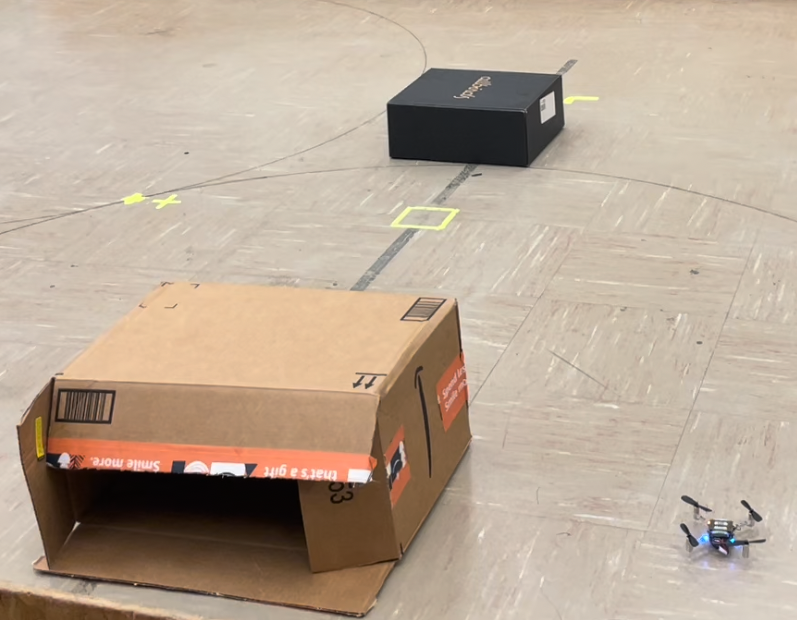
\includegraphics[width=0.5\linewidth]{Technical/OFG.png}  
  \caption{Object Filled Grid}
  \label{fig:OFG}
\end{figure}

\subsection{Milestones}
To ensure that the project was on track to be complete by the end of the semester, a series of milestones were developed to guide the team. Additionally, this helped to set intermediate goals, to allocate time efficiently, and to simplify the process of delegating tasks.

\subsubsection{Milestone 1: Determining Height Collection Method}
This milestone was to understand and implement how to get the absolute and relative z-position of the drone. There were two methods considered: using a loco-positioning system or using the z-position data of the drone. Once the latter method was selected, it was implemented in a flight test where the drone was flown in a straight line over an object of known height. The data was then extracted to see if the
drone was able to provide the x, y, and z position of the object. A visualization of this data is given below in Figure \ref{fig:m1}.

\begin{figure}[H]
  \centering
  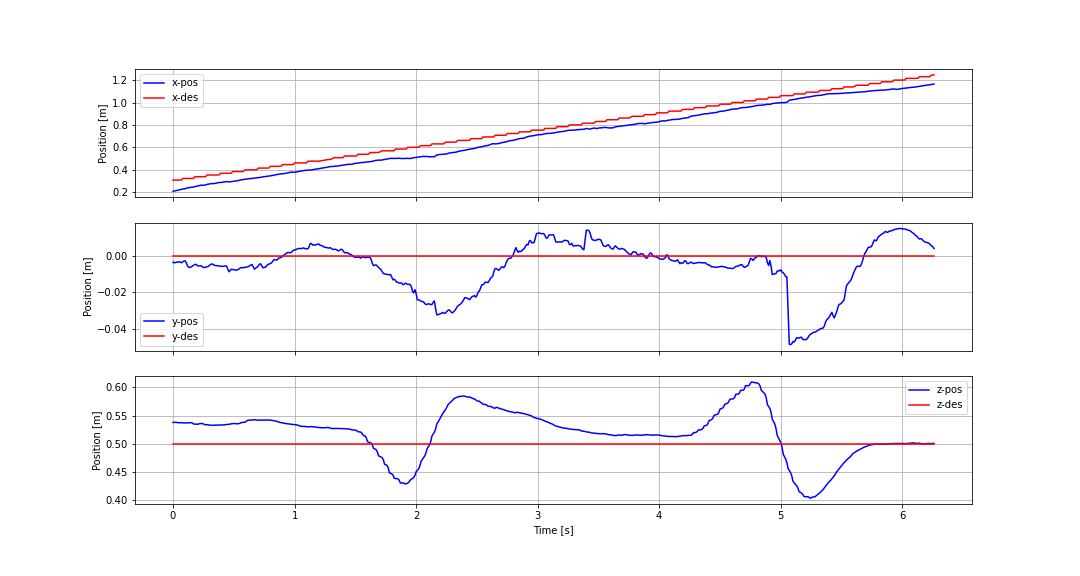
\includegraphics[width=1.0\linewidth]{Technical/m1.png}  
  \caption{Positional data versus time for straight line flight path over an object}
  \label{fig:m1}
\end{figure}

\subsubsection{Milestone 2: Map an Empty Grid}
This milestone was to have a successful flight in a lawnmower pattern over an empty grid and to visualize the topographical map of the empty grid. The topographic map of the empty grid is shown below in Figure \ref{fig:m2}.

\begin{figure}[H]
  \centering
  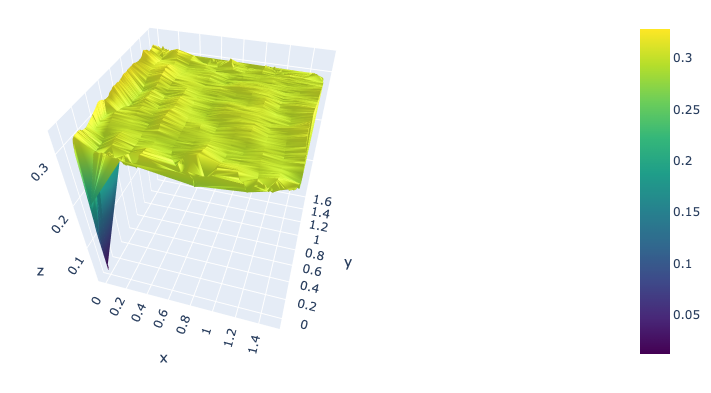
\includegraphics[width=0.8\linewidth]{Technical/m2.png}  
  \caption{Topographic map of empty grid}
  \label{fig:m2}
\end{figure}

\subsubsection{Milestone 3: Map an Object-filled Grid}
This milestone was to have a successful flight in a lawnmower pattern over an object-filled grid and to visualize the topographical map of the filled grid. This visualization is given below in Figure \ref{fig:m3}.

\begin{figure}[H]
  \centering
  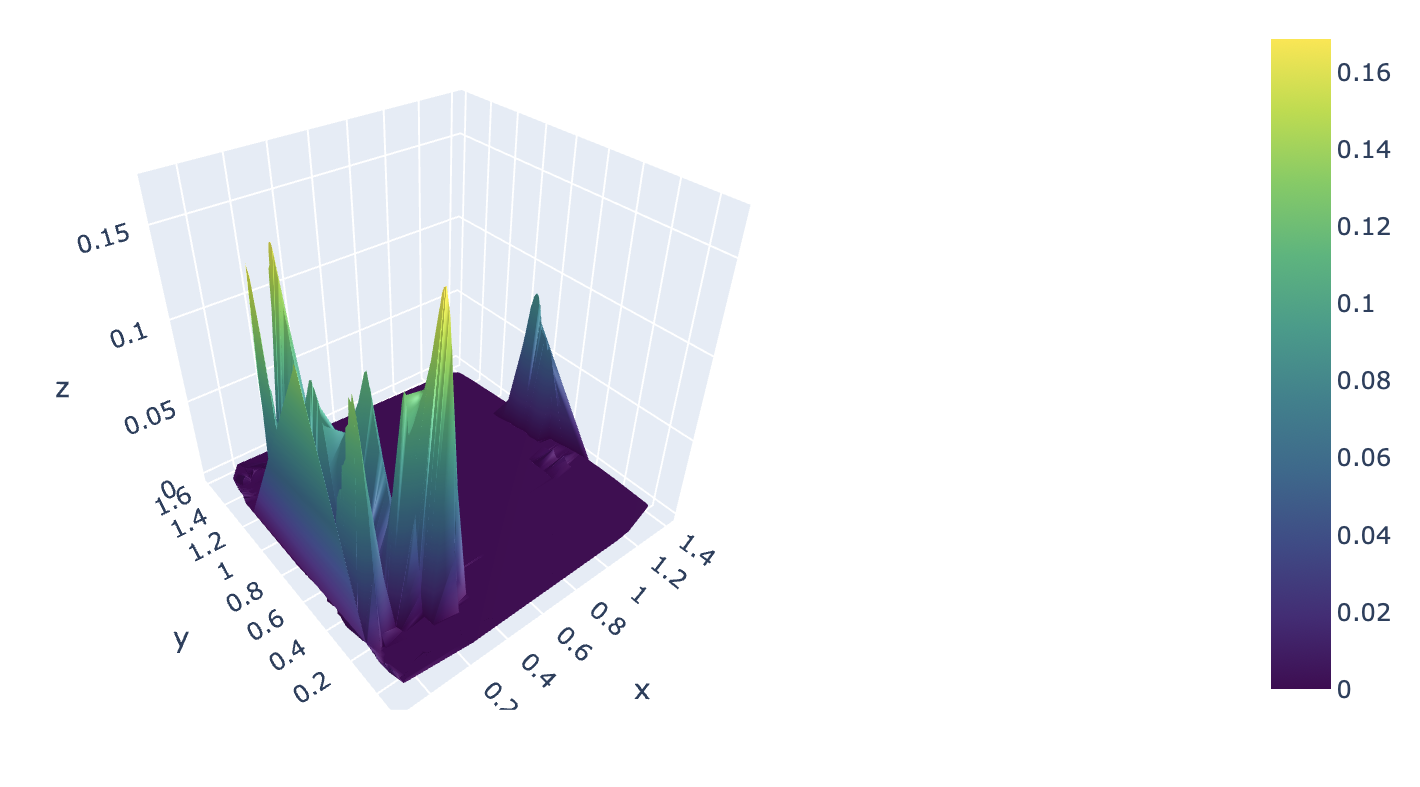
\includegraphics[width=0.8\linewidth]{Technical/m3.png}  
  \caption{Unprocessed topographic map of the object filled grid}
  \label{fig:m3}
\end{figure}

\subsubsection{Milestone 4: Visualization}
The final milestone was to produce the post-processed 3D topographical map of the object filled grid using Python. The produced visualizations were to be accurate replications of the real world object filled grid are shown and discussed in the results section.